\documentclass[a4paper]{sapthesis}
\usepackage{hyperref}
\usepackage{color}
\usepackage{graphicx}
\graphicspath{{./images/}}
\hypersetup{
    colorlinks,
    citecolor=black,
    filecolor=black,
    linkcolor=black,
    urlcolor=black,
}
\title{EEG signal denoising and arifact removal using \\ machine learning techniques}
\author{Martina Doku}
\IDnumber{1938629}
\course{Applied Computer Science and Artificial Intelligence}
\courseorganizer{Facoltà di Ingegneria dell’Informazione, Informatica e Statistica}
\AcademicYear{2022/23}
\advisor{Prof Danilo Avola}
\copyyear{2023}
\authoremail{doku.1938629@studenti.uniroma1.it}

\begin{document}
\maketitle
\dedication{dedication}
\begin{abstract}
This thesis aims to investigate the use of machine learning
 techniques for EEG signal denoising. The first part of the
thesis is dedicated to the introduction of the problem, the statement
of the research questions and an overview of the basic concepts.
The second part is dedicated to history and 
the state of
the art of signal analysis, and more specifically of the EEG signal
analysis and denoising methods. The third part is dedicated to the
 machine learning techniques.
The fourth part is dedicated to the experimental results and the last part
is dedicated to the conclusions and future works.
\end{abstract}
\tableofcontents
\chapter{Introduction}
The chapter is built as follows: in the first section there is a brief
introduction of the problem, the reasons that led to the choice of the
topic and the outline of the thesis. In the second section there is the
statement of the research questions. In the third section there is a brief
description of the basic concepts.
\section{Problem statement}
What is EEG in the first place and why is it important? Electroencephalography 
(EEG) is a non-invasive technique used to measure the electrical activity of
the brain. EEG signals are still among the less explored ones in the
field of signal processing, despite their widespread use in clinical 
practice and research. In recent years, there has been a growing 
interest in developing denoising methods for EEG data to improve their 
quality and reliability.\newline \\
The main objective of this thesis is to investigate and compare different
 EEG denoising methods, and to evaluate their performance in terms of 
 signal quality, artifact removal, and preservation of underlying brain
activity. Specifically, we will focus on the most recent machine learning
techniques, advanced models like the 'transformers'. We will also investigate the 
potential of combining different denoising methods to improve the 
performance of EEG denoising.\newline \\
Overall, this thesis aims to provide a better understanding of the strengths
 and limitations of different EEG denoising methods, and to help researchers
  and clinicians make informed decisions when selecting the most appropriate
   denoising method for their EEG data analysis. By improving the quality of
    EEG signals, we can enhance our understanding of brain function and 
    ultimately contribute to the development of more effective diagnostic 
    and therapeutic tools for neurological disorders.

\section{Research questions}
The research questions are the following:
\begin{itemize}
\item How can we remove artifacts from EEG signals?
\item How can we exploit the most recent machine learning techniques for
    EEG denoising?
\item What are the strengths and limitations of these new methods?
\item What are the performance of these new methods?
\end{itemize}
\section{Basic concepts}
In this section we will introduce the basic concepts that will be used 
in the thesis. The first part is dedicated to the EEG signal, the second
part is dedicated to the EEG denoising.
\subsection{EEG}
When talking about EEG,in this thesis, we are referring to the
electroencephalogram, in particular we are interested in the 
EEG waves. Electroencephalogram (EEG) waves are the patterns 
of electrical activity that are recorded by EEG measurements. 
These waves have different frequencies and amplitudes, and they 
reveal different states of brain activity. We divide the EEG waves in 
5 main categories depending on their frquency:Alpha, Beta, Theta, 
Delta and Gamma waves.\begin{figure}[h]
  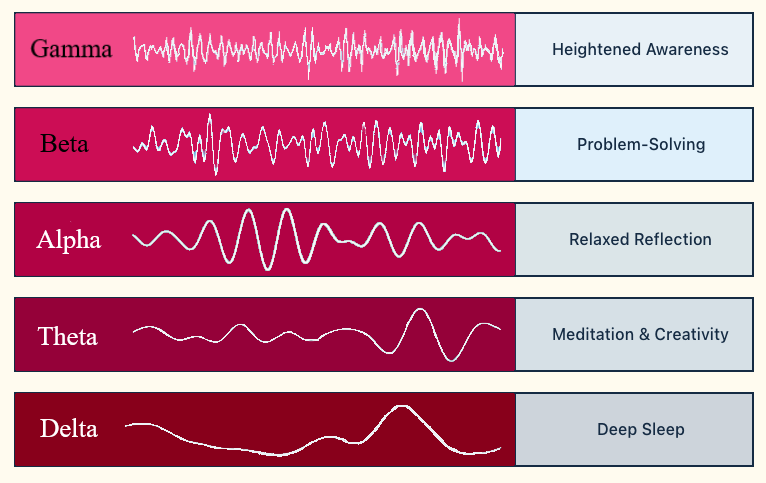
\includegraphics[scale=0.6]{waves}
  \centering
  \caption{Types of EEG waves}\label{fig:waves}
  
  \end{figure}\newline \\
Delta waves are typically observed during deep sleep and have a frequency
of less than 4 Hz. Theta waves are associated to light sleep or 
drowsiness and have a frequency of 4-7 Hz. Alpha waves correspond to the 
relaxed and awake state, witha frequency of 8-13 Hz. Beta waves, on the other 
hand, are associated with active cognitive processing and have a higher 
frequency of 14-30 Hz. Gamma waves have a frequency of 30-100 Hz and are associated with higher 
cognitive functions such as attention and memory.\newline \\
It's important to remember that EEG waves are not distinct entities but 
represent a continuous spectrum of activity that can be influenced by
various factors such as task demands, attention, and emotion. Interpreting EEG waves requires expertise 
and context since different patterns of EEG activity may reflect 
different states of brain activity depending on the individual and the 
experimental conditions. Furthermore, research has shown that EEG waves
can be useful in clinical diagnosis and prognosis, as well as in the
assessment of cognitive function and brain injury. Therefore, 
understanding the various EEG waves and their characteristics 
can provide valuable insights into brain function and activity.
\subsection{EEG denoising}
EEG signals can be influenced by various factor that alter the real waves 
originated from neural activities, those factors are defined as artifacts. 
The artifacts can be classified as\cite{EEG artifact}: 
\begin{itemize}
    \item intrinsic artifacts:
    artifacts that depend on physiological sources, such as ocular artifacts (EOG)
    that come from eye movement and blinking, muscle artifacts (EMG) and
     cardiac artifacts (ECG)
    \item extrinsic artifacts: artifacts generated from external electromagnetic 
    such as power line noise
    sources.
\end{itemize}
Denoising of EEG data is an essential task to be able to work on data and to
extract meaningful information from it. The denoising process is complex and
it does lead to different level of quality of the data depending on the 
method used, the quality of the data and the type of artifact.\\ \\
There are several challenges\cite{denoising challenges} related both 
to single methods characteristic and general artifact removal.
For example, some methods are computationally expensive and require a lot
of time to be applied, some methods are not able to remove all kind of
artifacts, some methods require a lot of data to be applied. On a general
level, there is the problem of the lack of a standard method to evaluate
the quality of the denoised data and the EEG applications are not 
yet fuly commercial, so there hasn't been a sufficient investment in
hardware and software to make the denoising process easier.\\ \\
However the main goal of latest studies is to find a method that can
denoise from all kind of artifacts and that can be used in a flexible
and fast way, to accomodate the needs of all the different EEG applications.
\chapter{Literature review}
In this chapter we will present the main methods used for the denoising
of EEG data. In the first part we will focus on the methods used for the
removal of artifacts from signals in general, in the second part we will
present the ones specifically deveolopped for the denoising of EEG data and in the third
part we will explore the latest, machine learning related, methods.
\section{Signal analysis}
In this section we will present the basic techniques used for the analysis
of signals that 
constituted a base for the ones developed for the analysis of EEG data.
\subsection{Fourier transform}\label{sec:fourier}
The first method used for the removal of artifacts from signals is the
Fourier transform\cite{fourier}. The Fourier transform is a mathematical tool used
 used to decompose a signal into sine and cosine functions, that are 
used as basis functions for the original signal.
It is defined as:

\begin{equation}\label{eq:fourier}
F(\omega) = \int_{-\infty}^{\infty} f(t) e^{-i\omega t} dt
\end{equation}

where $f(t)$ is the signal and $\omega$ is the frequency. The Fourier
transform of a signal is a complex number, which can be decomposed into
its real and imaginary parts. 

\subsection{Fast Fourier transform}\label{sec:fft}
The Fourier transform is a very useful tool for the analysis of signals,
but it is computationally expensive. The Fast Fourier transform (FFT)\cite{fft} is
an algorithm that is used to calculate the Fourier transform
of a signal in a shorter time: it reduces the time nedded to Nlog (N),
 obtaining a speed-up of a factor of N/log (N).\newline
The FFT is used  in many different fields of science such as
signal processing, image processing, etc\ldots
\begin{figure}[h]
  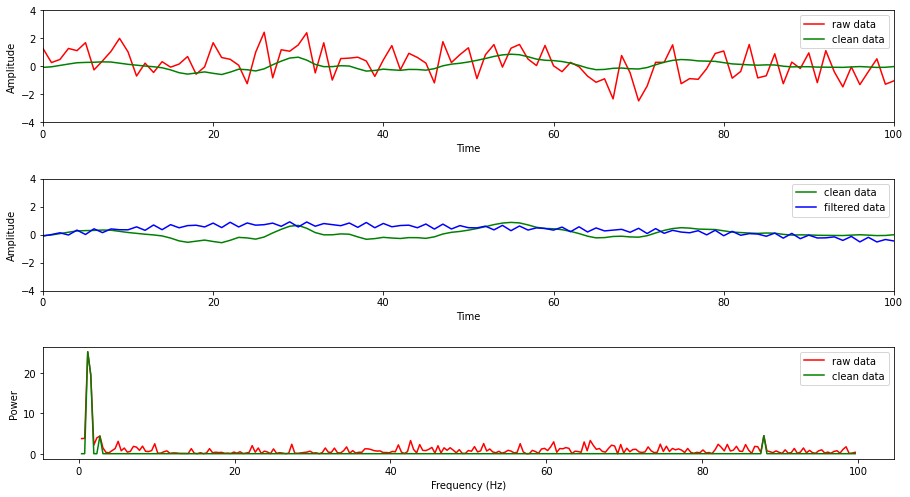
\includegraphics[scale=0.45]{fft_waves_result}
  \centering
  \caption{Result of the FFT of a signal
  }\label{fig:fft}
  
  \end{figure}
\subsection{Short Time Fourier Transform}\label{sec:stft}
The Short Time Fourier Transform (STFT)\cite{stft}\cite{stft2}
is a method used to calculate the
Fourier transform of a signal. It is used with non stationary signals
to find the frequency components of a signal over time.
The STFT equation is defined as:
\begin{equation}
\label{eq:stft}
S(\tau) = s(t) \cdot h(t-\tau)
\end{equation}
where $s(t)$ is the signal, $h(t)$ is the window function and $\tau$ is
the time. \newline
The STFT can be used to find the frequency components of a signal:
\begin{equation}
\label{eq:stft2}
S(\omega)= \frac{1}{2\pi}\cdot \int_{-\infty}^{\infty} s(\tau) \cdot h(t-\tau) e^{-i\omega t} d\tau
\end{equation}
where $s(\tau)$ is the signal, $h(t)$ is the window function and $\omega$
is the frequency. \newline
\begin{figure}[h]
  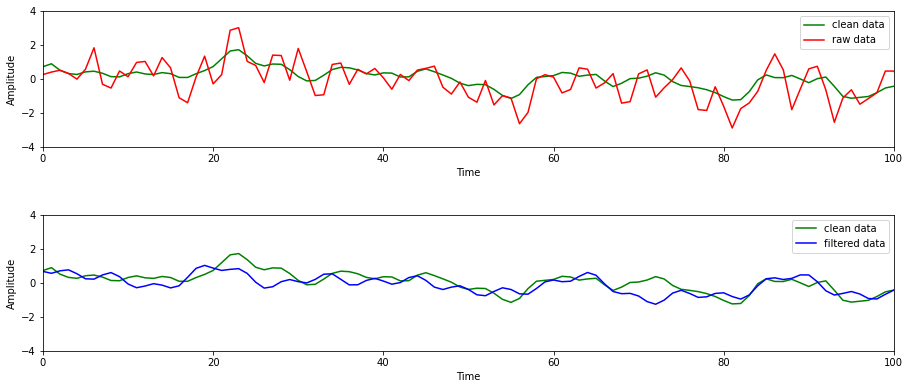
\includegraphics[scale=0.45]{stft_waves_result}
  \centering
  \caption{Result of the STFT of a signal
  }\label{fig:stft} 
  \end{figure}
\subsection{Wigner-Ville distribution}\label{sec:wvd}
The Wigner-Ville distribution (WVD)\cite{wvd} is a method used to provide
the description of a signal in the time-frequency domain with higher resolution.
It is described by the following equation:
\begin{equation}
\label{eq:wvd}
W(\tau, \omega) = \int_{-\infty}^{\infty} s(t-\tau) \cdot s^*(t-\tau) e^{-2\pi\omega \tau} d\tau
\end{equation}
where $s(t)$ is the signal, $\tau$ is the time and $\omega$ is the frequency.
The main problem of the WVD is that it introduces the so called cross terms.
In fact, for a signal
\begin{equation} x(t)=x_1(t)+x_2(t)
\end{equation}
the corresponding WVD is:
\begin{equation}
WVD(t,f)= WVDx_1(t,f) + WVDx_2(t,f) + 2Re[WVDx_1x_2(t,f)]
\end{equation}
where $2Re[WVDx_1x_2(t,f)]$ is the cross term
which is removable at the expense of a loss of resolution.  \newline
\begin{figure}[h]
  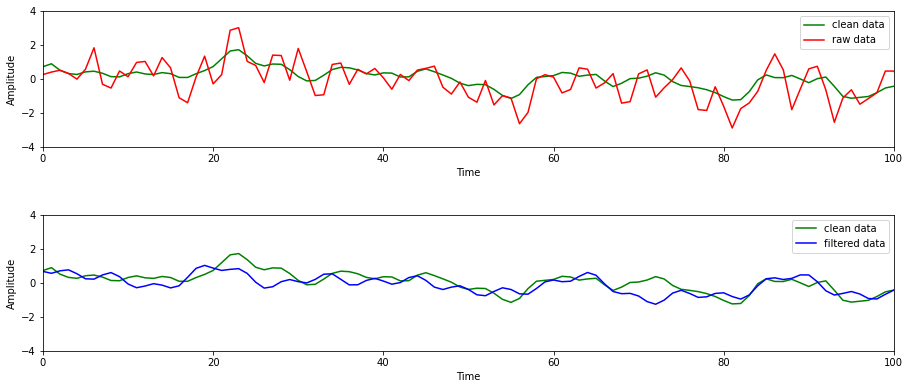
\includegraphics[scale=0.45]{wvd_waves_result}
  \centering
  \caption{Result of the WVD of a signal
  }\label{fig:wvd}
\end{figure}
\subsection{Wavelet transform}\label{sec:wavelet}
The wavelet transform\cite{wavelet} is a method used to find the frequency
components of a signal over time. It is used with non stationary signals and it
provides a better time-frequency resolution than the STFT and the WVD 
since it gives a better simultaneous time-frequency localization. \newline
It expresses the signal as a linear combination of mother wavelets.
The wavelet transform is defined as:
\begin{equation}
\label{eq:wavelet}
W(\tau, \omega) = \int_{-\infty}^{\infty} s(t-\tau) \cdot \psi(t-\tau) e^{-2\pi\omega \tau} d\tau
\end{equation}
where $s(t)$ is the signal, $\tau$ is the time, $\omega$ is the frequency
and $\psi(t)$ is the wavelet function. \newline
A possible choice for the wavelet function is the Morlet wavelet:
\begin{equation}
\label{eq:wavelet2}
\psi(t) = \frac{1}{\sqrt{2c\pi}} \cdot e^{-\frac{t^2}{2c^2}} \cdot e^{i\omega_0 t}
\end{equation}
where $\omega_0$ is the central frequency of the wavelet and $c$ is the
width of the wavelet. \newline

\subsection{Matching Pursuit}\label{sec:mp}
The Matching Pursuit (MP)\cite{mp} is a greedy algorithm used to approximate a
signal with a linear combination of basis functions called time-frequency 
atoms, selected from a dictionary of functions. \newline
A general family of time-frequency atoms can be generated by scaling, translating 
and modulating a single window function $g(t)$ as follows:
\begin{equation}
\label{eq:mp}
g_{\gamma}(t) = \frac{1}{\sqrt{s}} \cdot g(\frac{t-u}{s}) \cdot e^{i\xi t}
\end{equation}
where $\gamma$ is the tuple (s, u, $\xi$) $s$ is the scale, $u$ is the
translation and $\xi$ is the frequency modulation. \newline
The algorithm aims to find a set of atoms $\gamma_1, \gamma_2, \dots, \gamma_N$
that best approximate the signal $f(t)$, i.e.:
\begin{equation}
\label{eq:mp2}
f(t) \approx \sum_{i=1}^{N} a_i \cdot g_{\gamma}(t)
\end{equation}
where $a_i$ are the expansion coefficients. \newline
The vector f can be decomposed into 
\begin{equation}
\label{eq:mp3}
f(t) = <f, g_{\gamma}>g_{\gamma} + Rf(t)
\end{equation}
where $R_{f}$ is the residual vector after approximating f in the direction
 of $g_{\gamma}$. \newline
MP iteratively decomposes the residue $R_{f}$  by projecting it on a vector
of D that matches $R_{f}$ at best. \newline
\section{EEG denoising}\label{sec:denoising}
The denoising of EEG signals is performed using techniques developed from
the field of signal processing, but more suited to the specific characteristics
of EEG signals and artifacts. Here we present the most common methods.
\subsection{Regression}\label{sec:regression}
The regression method\cite{regression}, considers the EEG signal to be a
linear combination of the artifacts and the clean EEG signal. In particular,
the EEG signal is modeled as:
\begin{equation}
\label{eq:regression}
EEG = \alpha \cdot EMG + \beta \cdot EOG + \gamma \cdot ECG + \delta \cdot CEEG
\end{equation}
where $EEG$ is the registered EEG signal, $EMG$ is the muscle artifact
, $EOG$ is the ocular artifact,
$ECG$ is the cardiac artifact
and $CEEG$ is the clean EEG signal. \newline
The regression coefficients $\alpha, \beta, \gamma, \delta$ are estimated
using the least squares method. \newline
The regression method is simple and fast, but it doesn't take into account
the temporal correlation between the artifacts and the EEG signal, the so 
called cross terms. Furthermore it requires the knowledge of the artifacts
signals. \newline
\subsection{Blind source separation}\label{sec:bss}
Blind source separation (BSS)\cite{bss} is a  class of methods used to separate a
mixture of signals into their individual components. 
There are several BSS algorithms, all based on an unsupervised component 
separation. 
The most common BSS algorithms are the Principal Component Analysis (PCA),
the Principal Component Analysis (ICA) and the Canonical Correlation Analysis.
\newline

\subsubsection{Principal Component Analysis}
The PCA\cite{pca} is a method used to find a linear transformation of the
mixture signals that maximizes the variance of the transformed signals. 
First, data are standardized by subtracting the mean and dividing by the
standard deviation.
\begin{equation}
\label{eq:pca}
\textbf{Z} = (\textbf{X} - \textbf{m})/\textbf{s}
\end{equation}
Then, the covariance matrix is computed. 
\begin{equation}
\label{eq:pca2}
\textbf{C} = \frac{1}{n-1}\textbf{Z}^T\textbf{Z}
\end{equation}
The eigenvectors of the covariance matrix are the principal components of the data while the
eigenvalues are the variances of the principal components.
\begin{equation}
\label{eq:pca3}
\textbf{C}\textbf{v}_i = \lambda_i\textbf{v}_i
\end{equation}
The principal components found by projecting x onto those
 perpendicular basis vectors are uncorrelated, and their directions 
 orthogonal. This scheme is very efficient in redundancy reduction,
  and can be said to maximize the amount of information spanned by a
subset of dimensions of the initial vector. \newline

\subsubsection{Independent Component Analysis}
The ICA\cite{ica} is a method used to find a linear transformation of the
mixture signals that maximizes the non-Gaussianity of the transformed signals.
It consists in decomposing the signal in Independent components and 
discarding the ones containing artifacts. In blind source separation, the original independent
sources are assumed to be unknown, and we only have
access to their weighted sum.\cite{ica2} \newline
The signal is modeled as:
\begin{equation}
\label{eq:ica}
x(t) = \sum_{i=1}^{N} a_i \cdot s_i(t)
\end{equation}
where $x(t)$ is the mixture signal, $s_i(t)$ is the $i$-th source signal
and $a_i$ is the mixing coefficient. \newline
The ICA algorithm aims to find the source signals $s_i(t)$ and the mixing
coefficients $a_i$ that maximize the non-Gaussianity of the mixture signal
$x(t)$. 
It is based on the assumption that the sources are statistically independent.
\newline

\subsubsection{Canonical Correlation Analysis}
The CCA\cite{cca} is a method used to find a linear transformation of the
mixture signals that maximizes the correlation between the transformed signals.
More specifically, CCA identifies two sets of variables, X and Y, and 
finds linear combinations of X and Y that are maximally correlated. 
These linear combinations are called canonical variates.
 The first canonical variate is the linear combination of X and Y that 
 has the highest correlation, and each subsequent canonical variate is 
 the linear combination that has the highest correlation subject to being
  orthogonal to the previous canonical variates.
\newline

\subsection{Empirical Mode Decomposition}\label{sec:emd}
The EMD\cite{emd} is a method used to decompose a signal into a set of
intrinsic mode functions (IMFs). The EMD is a data-driven method that
does not require any prior knowledge of the signal. \newline
It decomposes a signal into a finite number of intrinsic mode functions
 (IMFs), which are functions that capture the local behavior of the signal.
  EMD is based on the concept of sifting, which involves iteratively
 extracting the local maxima and minima of the signal to generate IMFs.
The basic steps of EMD are as follows:
\begin{itemize}
    \item Given a signal $x(t)$, find all of its local maxima and minima.
    \item Interpolate between the local maxima and minima to create an
    upper and lower envelope for the signal. This step effectively
     eliminates the high-frequency components of the signal and 
     captures its slowly varying behavior.
    \item Calculate the mean of the upper and lower envelopes to obtain a
     first IMF, $c_1(t)$.
    \item Subtract $c_1(t)$ from the original signal to obtain a new signal,
        $r_1(t) = x(t) - c_1(t)$.
    \item Repeat steps 1-4 on the residual signal $r_1(t)$ to obtain the
        second IMF, $c_2(t)$.
    \item Continue this process until a stopping criterion is met, such as
        the number of IMFs or the amplitude of the residual signal falling
        below a certain threshold.
\end{itemize}
The resulting IMFs are functions that oscillate around zero with a 
characteristic scale and capture the local behavior of the signal at 
different scales. The final residual signal is a monotonic function that 
represents the long-term trend of the signal.
\subsection{Filtering techniques} \label{sec:filtering}
\subsubsection{Adaptive filtering}
Adaptive filtering\cite{adaptive} is a method used to estimate the
unknown input signal from the noisy output signal. It is based on the
assumption that the input signal is a linear combination of the unknown
input signal and the noise. \newline
The basic steps of adaptive filtering are as follows:
\begin{itemize}
    \item Given a noisy signal $y(t)$, estimate the unknown input signal
    $x(t)$.
    \item Initialize the filter coefficients $w_0$.
    \item For each sample $y(t)$, compute the error signal $e(t)$.
    \item Update the filter coefficients $w(t)$.
    \item Repeat steps 2-4 until a stopping criterion is met.
    
\end{itemize}
The error signal is defined as the difference between the noisy signal
and the estimated input signal. The filter coefficients are updated
according to the following equation:
\begin{equation}
\label{eq:adaptive}
w(t+1) = w(t) + \mu \cdot e(t) \cdot x(t)
\end{equation}
where $\mu$ is the step size. \newline

\subsubsection{Wiener filtering}
Wiener filtering\cite{wiener} is a method used to estimate the unknown
input signal from the noisy output signal. It is based on the assumption
that the input signal is a linear combination of the unknown input signal
and the noise. \newline
The basic steps of Wiener filtering are as follows:
\begin{itemize}
    \item Given a noisy signal $y(t)$, estimate the unknown input signal
    $x(t)$.
    \item Compute the power spectral density (PSD) of the noise signal
    $n(t)$.
    \item Compute the PSD of the input signal $x(t)$.
    \item Compute the PSD of the output signal $y(t)$.
    \item Compute the Wiener filter coefficients $w(t)$.
    \item Apply the Wiener filter to the noisy signal $y(t)$ to obtain the
    estimated input signal $x(t)$.
\end{itemize}
The Wiener filter coefficients are computed according to the following
equation:
\begin{equation}
\label{eq:wiener}
w(t) = \frac{S_x(t)}{S_x(t) + S_n(t)}
\end{equation}
where $S_x(t)$ is the PSD of the input signal $x(t)$ and $S_n(t)$ is the
PSD of the noise signal $n(t)$. \newline



\section{Machine learning}
The latest approaches involve the use of machine learning techniques
to denoise EEG signals. Machine learning is a subfield of artificial
intelligence that focuses on the development of computer programs that
can learn from data. In the following chapter we will discuss the
different architectures of neural networks that have been used in 
previous works and that will be exploited in the proposed approach.
\subsection{Fully connected neural network}
Fully Connected Neural Networks, also known as Feedforward Neural Networks
or Multilayer Perceptrons, are the the most common type of neural networks.
They consist of neurons[\ref{sec:neuron}], organized in layers and each of
 the neurons in a layer
 is connected to all the ones in the previous and subsequent layers. 
These connections are weighted, and each neuron computes a weighted sum of its inputs, passes
  this sum through an activation function, and then forwards the result to
 the next layer.\newline \\
The architecture of a Fully Connected Neural Network consists of one or
 more layers of neurons, including an input layer, one or more hidden 
 layers, and an output layer. The input layer receives the data to be
  processed, and each neuron in this layer represents a feature of the 
  input. The hidden layers perform complex computations on the input data,
and the output layer produces the final output of the network. The 
number of neurons in the input and output layers is determined by the
size of the input and output data, while the number of neurons in the
hidden layers is a hyperparameter that can be tuned to improve the
performance of the network.
\begin{figure}[h]
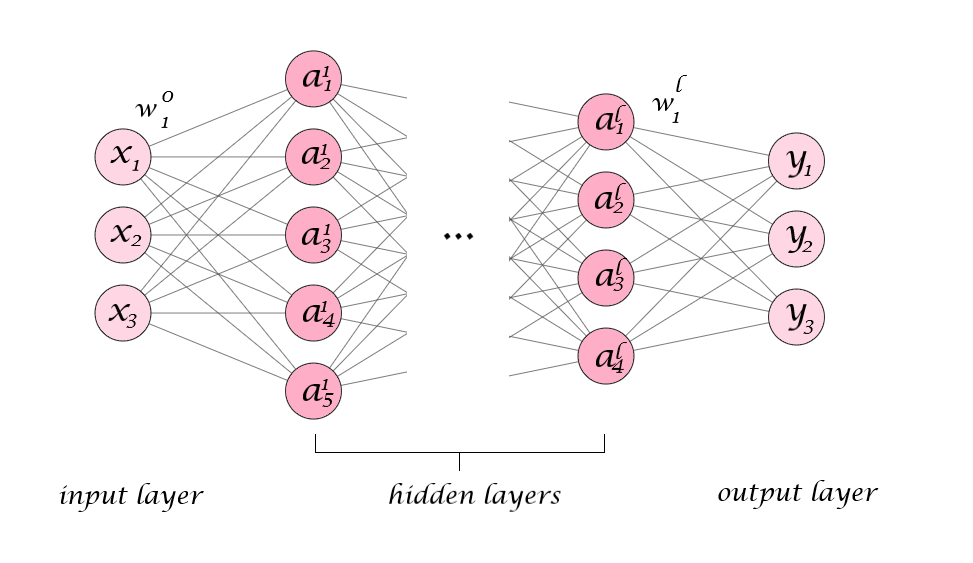
\includegraphics[scale=0.5]{fully_connected_nn}
\centering
\caption{Fully connected neural network}\label{fig:fully_connected}

\end{figure}\newline \\
The operation of a fully connected neural network can be described 
mathematically using the following equations.
\subsubsection{Linear transformation}
Each neuron in the hidden layers and output layer
 performs a linear transformation of its inputs, which is a weighted sum 
 of the outputs of the neurons in the previous layer. The linear 
 transformation of neuron i in layer l can be expressed as:
 \begin{equation}
  \label{eq:linear_transformation}
z_i^l = \sum_{j=1}^{n^{l-1}} w_{ij}^l a_j^{l-1} + b_i^l
\end{equation}
where $n^{l-1}$ is the number of neurons in the previous layer,
 $w_{ij}^l$ is the weight of the connection between neuron j in layer 
 l-1 and neuron i in layer l, $a_j^{l-1}$ is the output of neuron j 
 in layer l-1, $b_i^l$ is the bias term of neuron i in layer l, and
  $z_i^l$ is the pre-activation value of neuron i in layer l.
  \subsubsection{Activation function}
The pre-activation values of each neuron are 
passed through an activation function to introduce non-linearity
 into the network. Commonly used activation functions include sigmoid,
  tanh, ReLU, and softmax. The activation function of neuron i in layer
l can be expressed as:
\begin{equation}
\label{eq:activation_function}
a_i^l = \sigma(z_i^l)
\end{equation}
where $\sigma$ is the activation function.
\subsubsection{Output computation}
 The output of the network is produced by the output
 layer, which applies a final activation function to the pre-activation
  values of its neurons. The activation function of the output layer 
  depends on the task the network is designed to perform. The output of neuron i in the output layer can be expressed as:
\begin{equation}
\label{eq:output}
  \hat{y_i} = \sigma(z_i^L)
\end{equation}
where L is the index of the output layer, $\sigma$ is the output activation
 function, and $\hat{y_i}$ is the predicted value of the i-th output.\newline \\
The network is trained by adjusting the weights and biases using
backpropagation [\ref{sec:backpropagation}] with respect to a loss function
 [\ref{sec:loss}].

\subsection{Convolutional neural network}
Convolutional Neural Networks (CNNs) are a type of artificial neural network
 architecture commonly used in deep learning for multidimensional data
  analysis.
Unlike fully connected neural networks, CNNs take into account the spatial
structure of input data, such as images, by using convolutional layers 
that apply filters to local regions of the input.\newline \\
The architecture of a CNN consists of one or more convolutional layers paired 
with their activation functions,
followed by one or more fully connected layers. The convolutional layers 
perform feature extraction by applying filters to local regions of the 
input data, producing feature maps that highlight different aspects of 
the input data. The fully connected layers perform classification or
 regression on the feature maps produced by the convolutional layers.\begin{figure}[h]
  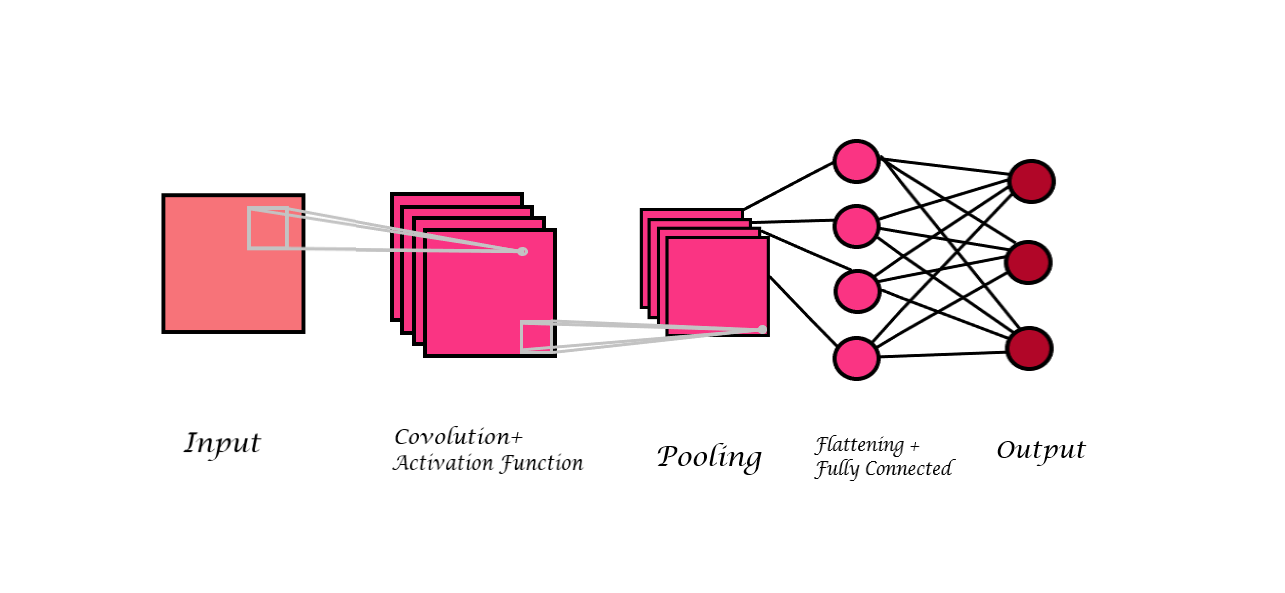
\includegraphics[scale=0.5]{convolution_nn}
  \centering
  \caption{Convolutional neural network}\label{fig:convolution_nn}
  \end{figure}\newline \\
The operation of a CNN can be described mathematically using the following
equations:
\subsubsection{Convolutional layer}
In the convolutional layers, a set of filters or kernels is 
applied to local regions of the input data to produce feature maps. The 
convolution operation can be expressed as:
\begin{equation}
  \label{eq:convolution}
  z_{i,j,k} = \sum_{l=1}^{d_{in}}\sum_{m=1}^{f}\sum_{n=1}^{f} x_{i+m-1,j+n-1,l}w_{m,n,l,k} + b_k
\end{equation}
where $x$ is the input data, $w$ is the filter, $b$ is the bias, $d_{in}$ 
is the number of input channels, $f$ is the size of the filter, $z$ is the 
output feature map, and $i,j,k$ are the indices of the feature map. 
\subsubsection{Pooling layer}
The pooling layer downsamples the output of the convolutional 
layer, reducing the size of the feature maps and introducing translation
 invariance. Commonly used pooling operations include max pooling and
average pooling that perform a max or average operation on local regions
 of the input data, respectively.
\subsubsection{Flattening}
The output of the pooling layer is flattened into a
 single vector, with dimension equal to the number of neurons of the
 input layer of the fully connected part of the network,
 to which it is passed.
\subsubsection{Fully connected layer}
The fully connected layers perform classification
 or regression on the feature maps produced by the convolutional and
  pooling layers. The operation of a fully connected layer is similar 
  to that of a fully connected neural network.
\subsection{Long short-term memory}
Long Short-Term Memory (LSTM) Networks are a type of recurrent neural 
network (RNN) specifically designed to address the vanishing 
gradient problem[\ref{sec:vanishing_gradient}] in traditional RNNs. LSTMs have a memory cell that is
 able to maintain information over long periods of time, and they use 
 three gates - the input gate, the forget gate, and the output gate -
  to regulate the flow of information into and out of the memory cell.
  \begin{figure}[h]
    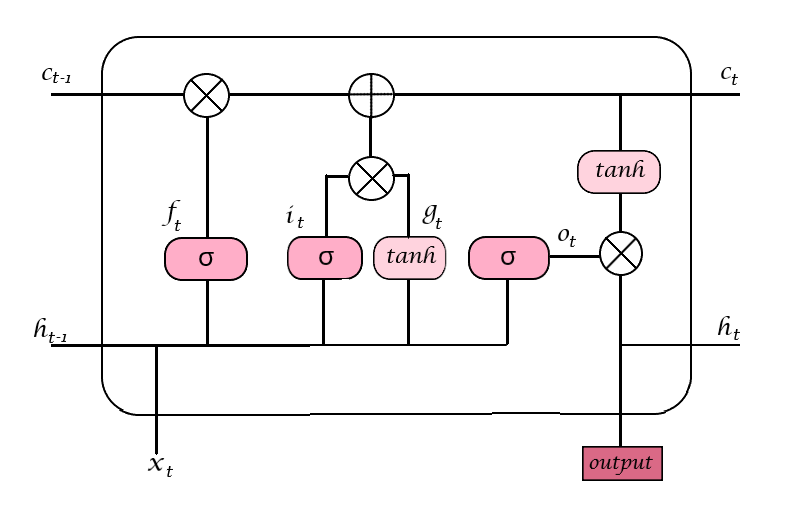
\includegraphics[scale=0.5]{lstm}
    \centering
    \caption{Long Short Term Memory Architecture}\label{fig:lstm}
    \end{figure} 
Here are the key equations that govern the behavior of an LSTM:
\subsubsection{Input gate}
The input gate determines how much of the new input should be added to the 
memory cell. The equation for the input gate is:
\begin{equation}
  i_t = \sigma(W_i [h_{t-1}, x_t] + b_i)
  \end{equation}
where $i_t$ is the input gate activation vector, $x_t$ is the input vector 
at time t, $h_{t-1}$ is the hidden state vector from the previous time 
step, $W_i$ is the weight matrix for the input gate, and $b_i$ is the bias 
vector for the input gate.
\subsubsection{Forget gate}
The forget gate determines how much of the previous memory cell state 
should be retained. The equation for the forget gate is:
\begin{equation}
  f_t = \sigma(W_f [h_{t-1}, x_t] + b_f)
  \end{equation}
where $f_t$ is the forget gate activation vector, $x_t$ is the input 
vector at time t, $h_{t-1}$ is the hidden state vector from the previous time
 step, $W_f$ is the weight matrix for the forget gate, and $b_f$ is the bias 
 vector for the forget gate.
\subsubsection{Candidate memory cell state}
The memory update combines the input with the previous memory cell
 state to create a new memory cell state. The equation for the
  memory update is:
  \begin{equation}
    g_t = \tanh(W_g [h_{t-1}, x_t] + b_g)
    \end{equation}
where $g_t$ is the candidate memory cell state, $x_t$ is the input vector 
at time t, $h_{t-1}$ is the hidden state vector from the previous time step,
 $W_g$ is the weight matrix for the memory update, and $b_g$ is the bias vector
  for the memory update.
\subsubsection{Output gate}
The output gate determines how much of the new memory cell state should be 
output. The equation for the output gate is:
\begin{equation}
  o_t = \sigma(W_o [h_{t-1}, x_t] + b_o)
  \end{equation}
where $o_t$ is the output gate activation vector, $x_t$ is the input vector
 at time t, $h_{t-1}$ is the hidden state vector from the previous time step,
  $W_o$ is the weight matrix for the output gate, and $b_o$ is the bias vector 
  for the output gate.
\subsubsection{Hidden state update}
The new memory cell state is combined with the output gate
 to create the new hidden state. The equation for the hidden state update is:
 \begin{equation}
  h_t = o_t \tanh(c_t)
  \end{equation}
where $h_t$ is the new hidden state, $o_t$ is the output gate activation vector,
 $c_t$ is the new memory cell state, and tanh is the hyperbolic tangent function.\newline \\
These equations allow an LSTM network to selectively forget or remember
 information over time, making it well-suited for modeling sequences of
  data where long-term dependencies are important

\subsection{Transformer}
The Transformer is a neural network architecture designed for natural
 language processing tasks. It was introduced in the paper "Attention
  is All You Need" by Vaswani et al. in 2017\cite{attention}, and has since become 
  a popular choice for many NLP and sequential data tasks.\newline \\
 The Transformer
   is a type of encoder-decoder architecture, where the encoder is used 
   to encode the input sequence into a fixed-length vector, and the 
   decoder is used to decode the vector into an output sequence, both 
   encoder and decoder parts are composed of a stack of one of more layers.
    Each layer is composed of a multi-head self-attention mechanism, followed 
  by a position-wise fully connected feed-forward network.\newline
\begin{figure}[h]
  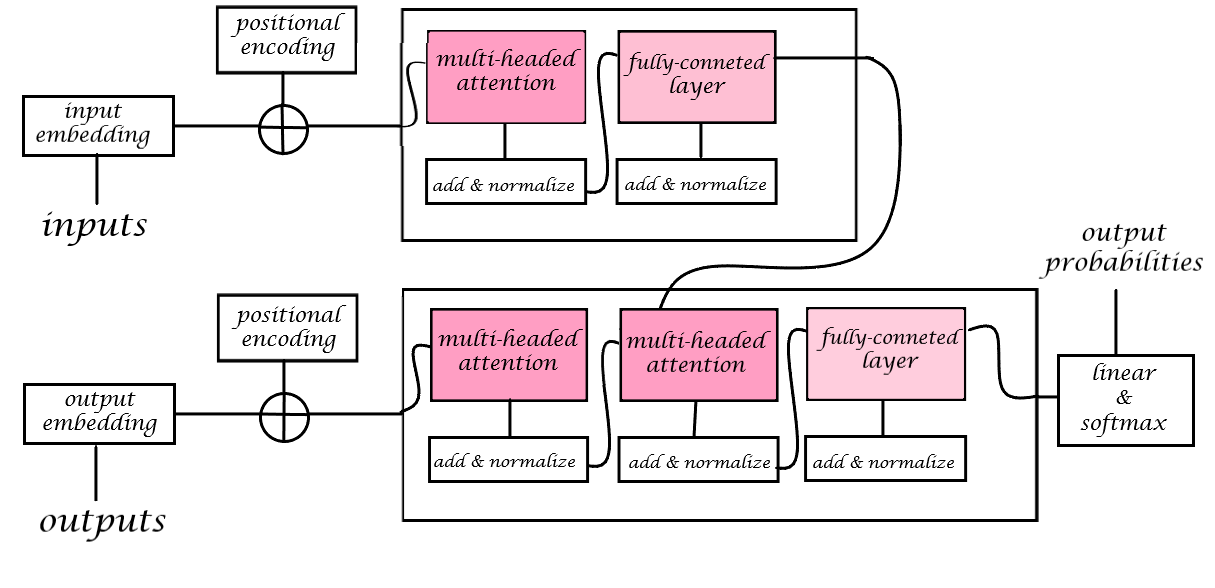
\includegraphics[scale=0.42]{transformer}
  \centering
  \caption{Transformer Architecture}\label{fig:transformer}
  \end{figure}
We will now go over the different components of the Transformer in more
 detail.
\subsubsection{Embedding}
The embedding layer precedes the encoder (and decoder) parts, it is used to convert 
the input sequence (or output sequence) into a vector
 representation. It is composed of two parts: an 
 embedding matrix, and a positional encoding matrix. The embedding matrix
  is used to convert the input sequence into a vector representation, and
   the positional encoding matrix is used to encode the position of each 
   token in the sequence. The embedding layer is defined as follows:
   \begin{equation}
     E = W_eX + W_p
     \end{equation}
where $X$ is the input sequence, $W_e$ is the embedding matrix, $W_p$ is the
 positional encoding matrix, and $E$ is the embedding vector.
\subsubsection{Self-attention}
The self-attention mechanism allows the model to 
attend to different parts of the input sequence. Given an input sequence,
we define the query, key, and value vectors as follows:
\begin{equation}
  Q = W_qX
  \end{equation}
\begin{equation}
  K = W_kX
  \end{equation}
\begin{equation}
  V = W_vX
  \end{equation}
where $X$ is the input sequence, $W_q$, $W_k$, and $W_v$ are the weight
  matrices for the query, key, and value vectors, respectively, and $Q$,
  $K$, and $V$ are the query, key, and value vectors, respectively. 
  
  Those values are then used to compute the attention scores as follows:
  \begin{equation}
    A = \text{softmax}\left(\frac{QK^T}{\sqrt{d_k}}\right)
    \end{equation}
where $A$ is the attention matrix, $d_k$ is the dimensionality of the
  key vectors, and $\text{softmax}$ is the softmax function. The 
  attention matrix is then used to compute the output vectors as follows:
  \begin{equation}
    O = AV
    \end{equation}
where $O$ is the output matrix. 
\subsubsection{Multi-head attention}
The multi-head attention mechanism allows the model to attend to different
 aspects of the input sequence simultaneously. It does this by 
computing $h$ different sets of query, key, and value vectors,
each of which is obtained by projecting the input vectors into
$d_k$, $d_k$, and $d_v$-dimensional spaces, respectively. 
The resulting $h$ sets of output vectors are concatenated
 and linearly transformed to produce the final output.\newline
 The equations for the multi-head attention mechanism can be written as 
 follows:
 \begin{align*}
 \text{MultiHead}(Q,K,V) &= \text{Concat}(head_1,\ldots,head_h)W^O \
\end{align*}
where:
 \begin{align*}
   head_i &= \text{Attention}(QW_i^Q, KW_i^K, VW_i^V)
 \end{align*}
 where $W_i^Q$, $W_i^K$, and $W_i^V$ are learned projection matrices for
  the $i$-th head, each of which has dimensions $d_{model}\times d_k$,
   $d_{model}\times d_k$, and $d_{model}\times d_v$, respectively.
    $W^O$ is a learned projection matrix that maps the concatenated
 output of the attention heads back to the original dimensionality of
  the input.
\subsubsection{Add and normalize}
The add and normalize layer is used to add the input to the output of the
  multi-head attention mechanism, and then normalize the result. The
    equations for the add and norm layer can be written as follows:
    \begin{align*}
      \text{AddNorm}(x,y) &= \text{LayerNorm}(x+y) \\
      \text{LayerNorm}(x) &= \text{Norm}(x+\text{Sublayer}(x))
      \end{align*}
where $x$ is the input vector, $y$ is the output of the multi-head
  attention mechanism, and $\text{Sublayer}(x)$ is the sublayer that
    is being normalized.
\subsubsection{Position-wise feed-forward network}
The position-wise feed-forward network is a simple two-layer neural 
network that operates on each position of the input sequence 
independently. It is applied to each output vector of the self-attention
 mechanism, and has the effect of transforming the vector into a 
 higher-dimensional space, followed by a projection back into the
  original dimensionality.\newline
The equations for the position-wise feed-forward network can be written
 as follows:
 $$\text{FFN}(x) = \text{ReLU}(xW_1+b_1)W_2+b_2$$
 In this equation, $x$ is the input vector of size $d_{model}$,
  $W_1$ and $W_2$ are learned weight matrices of sizes 
  $d_{model}\times d_{ff}$ and $d_{ff}\times d_{model}$,
respectively, $b_1$ and $b_2$ are learned bias vectors of
size $d_{ff}$ and $d_{model}$, respectively, and ReLU is the
rectified linear unit activation function. The output of the
position-wise feed-forward network is also a vector of size $d_{model}$.
\subsubsection{Linear and softmax}
The linear and softmax layer is used to convert the output of the decoder
 into a probability distribution over the target vocabulary. The equations for the
   linear and softmax layer can be written as follows:
   \begin{align*}
     \text{Linear}(x) &= xW+b \\
     \text{Softmax}(x) &= \text{softmax}(x)
     \end{align*}
where $x$ is the input vector, $W$ is the learned weight matrix, and $b$
  is the learned bias vector.
\chapter{Methodology}
\section{Data}\label{sec:data}
The data used in this thesis are the EEG signals of the EEGdenoiseNet 
dataset\cite{EEGdenoiseNet}. It is comprehensive benchmark dataset
 that proves to be an exemplary resource for training and evaluating
  deep learning-based EEG denoising models. It is composed of 4514 clean 
  EEG epochs, 3400 EOG epochs, and 5598 EMG epochs, making it an inclusive 
  and extensive dataset that caters to the needs of researchers and
 practitioners alike.\newline \\
The incorporation of these various types of epochs in the dataset
enables to generate a considerable number of noisy EEG epochs
with their corresponding ground truth data. As a result, this compilation 
has proven to be an invaluable resource for model training and testing,
 facilitating an enhanced understanding of EEG denoising.
\section{Preprocessing}
The preprocessing of the EEG signals is an important step in the
pipeline of the proposed model. It is used to generate the noisy EEG
signals that are used as input to the model.
The processing step used is proposed by the authors of the EEGdenoiseNet
dataset\cite{EEGdenoiseNet}. It is a simple yet effective method that
is used to generate noisy EEG signals from the clean EEG signals and clean 
EMG and EOG signals present in the dataset.
The preprocessing step is performed as follows:
\begin{enumerate}
\item The clean EEG signals and noise signals are augmented adding 
random disturb
\item The EEG signals are partially reused to match the EMG and EOG
signals
\item Data are divided in training, validation, and test sets
\item The noise signals are added to the EEG signals
\item The noisy EEG signals are normalized by dividing them by the
standard deviation
\end{enumerate}
At the end of the preprocessing step, the dataset is composed of:
\begin{itemize}
\item 44780 training EMG contaminated EEG samples
\item 5600 validation EMG contaminated EEG samples
\item 5600 test EMG contaminated EEG samples
\item 27200 training EOG contaminated EEG samples
\item 3400 validation EOG contaminated EEG samples
\item 3400 test EOG contaminated EEG samples
\end{itemize}
\section{Denoising}
\section{Machine learning}
\chapter{Experimental results}
\section{Results}
\section{Discussion}
\chapter{Conclusions and future work}
\section{Conclusions}
\section{Future work}
\chapter{Appendix}
\section {Neural network}
\subsection{Neuron}\label{sec:neuron}
A neuron, also known as a node or a perceptron, is a fundamental building
 block of a neural network. It is a mathematical function that receives one
or more inputs and produces an output based on those inputs. \newline 
A typical neuron in a neural network consists of three main components:\newline \\
Inputs: These are the signals or information that the neuron receives from 
other neurons or from the outside world.
 Each input is assigned a weight, which determines how important it is 
 to the neuron's output. \newline \\
Activation Function: The activation function is a non-linear function 
that takes the weighted sum of the inputs and produces an output. 
The output of the activation function is then passed on to the next 
layer of neurons in the network.\newline \\
Bias: The bias is an additional input that is used to adjust the output 
of the activation function. It can be thought of as a threshold that the 
weighted sum of the inputs must cross before the neuron "fires" or 
produces an output.
\subsection{Loss function} \label{sec:loss}
A loss function is a mathematical function that measures the difference 
between the predicted output of the network and the actual output (or 
"ground truth") for a given set of input data.\newline 
The goal of a neural network is typically to minimize the difference 
between the predicted output and the ground truth. The loss function 
provides a quantitative measure of this difference, which the network 
can use to adjust its parameters (such as the weights and biases of the 
neurons) in order to improve its predictions.\newline 
There are many different types of loss functions that can be used in a 
neural network, depending on the specific task the network is trying to 
perform. Some common examples include:
\begin{itemize}
\item{Mean Squared Error (MSE)}: This is a popular loss function for regression 
problems, where the goal is to predict a continuous output value. It 
measures the average squared difference between the predicted and actual 
values.
\item{Binary Cross-Entropy}: This is a loss function that is commonly used for 
binary classification problems, where the goal is to predict a binary 
output (e.g., 0 or 1). It measures the difference between the predicted 
probability of the positive class and the true probability (which is 
either 0 or 1).
\item{Categorical Cross-Entropy}: This is a loss function that is commonly used 
for multi-class classification problems, where the goal is to predict one 
of several possible output classes. It measures the difference between the 
predicted probability distribution over the classes and the true 
distribution (which is typically represented as a one-hot encoded vector).
\end{itemize}
By minimizing the loss function during training, the neural network 
can adjust its parameters to improve its predictions on the training 
data. However, it's important to also evaluate the performance of the 
network on a separate set of validation or test data to ensure that 
it is not overfitting to the training data.
\subsection{Backpropagation}\label{sec:backpropagation}
 The weights and biases of the network are updated during 
training using an algorithm called backpropagation, which computes the 
gradient of the loss function with respect to the network parameters.
 The gradient is then used to update the weights and biases of the network
  using an optimization algorithm such as stochastic gradient descent.

\subsection{Vanishing gradient problem}\label{sec:vanishing_gradient}
The vanishing gradient problem is a common problem in deep neural networks
 that occurs when the gradient of the loss function with respect to the
  weights and biases of the network is very small. This problem can be 
  solved by using a different activation function, such as the rectified 
  linear unit (ReLU) activation function, which does not suffer from the 
  vanishing gradient problem.
\begin{thebibliography}{1}
    \bibitem{EEG artifact}{Jiang, X.; Bian, G.-B.; Tian, Z. Removal of Artifacts from EEG Signals: A Review. Sensors 2019, 19, 987.}
    \bibitem{denoising challenges}{Wajid Mumtaz, Suleman Rasheed, Alina Irfan, Review of challenges associated with the EEG artifact removal methods, Biomedical Signal Processing and Control, Volume 68, 2021, 102741, ISSN 1746-8094}
    \bibitem{fourier} {Boashash, B., ed. (2003), Time–Frequency Signal Analysis and Processing: A Comprehensive Reference, Oxford: Elsevier Science, ISBN 978-0-08-044335-5.}
    \bibitem{fft} {Cooley, James W. (1987). The Re-Discovery of the Fast Fourier Transform Algorithm (PDF). Microchimica Acta. Vol. III. Vienna, Austria. pp. 33–45. Archived (PDF) from the original on 2016-08-20.}
    \bibitem{stft} {R. Álvarez, E. Borbor and F. Grijalva, ''Comparison of methods for signal analysis in the time-frequency domain,'' 2019 IEEE Fourth Ecuador Technical Chapters Meeting (ETCM), 2019, pp. 1-6, doi: 10.1109/ETCM48019.2019.9014860.}
    \bibitem{stft2} {W. -k. Lu and Q. Zhang, "Deconvolutive Short-Time Fourier Transform Spectrogram," in IEEE Signal Processing Letters, vol. 16, no. 7, pp. 576-579, July 2009, doi: 10.1109/LSP.2009.2020887.}
    \bibitem{wvd} {E. Chassande-Mottin and A. Pai, "Discrete time and frequency Wigner-Ville distribution: Moyal's formula and aliasing," in IEEE Signal Processing Letters, vol. 12, no. 7, pp. 508-511, July 2005, doi: 10.1109/LSP.2005.849493}
    \bibitem{wavelet}{ S. Zhou, B. Tang and R. Chen, "Comparison between Non-stationary Signals Fast Fourier Transform and Wavelet Analysis," 2009 International Asia Symposium on Intelligent Interaction and Affective Computing, Wuhan, China, 2009, pp. 128-129, doi: 10.1109/ASIA.2009.31.}
    \bibitem{wavelet2}{ V. M. Pukhova and M. S. Stepanova, "Up-Chirplet and Down-Chirplet Transforms of Non-Stationary Signals," 2019 IEEE Conference of Russian Young Researchers in Electrical and Electronic Engineering (EIConRus), Saint Petersburg and Moscow, Russia, 2019, pp. 1221-1225, doi: 10.1109/EIConRus.2019.8657179.}
    \bibitem{mp} {S. G. Mallat and Zhifeng Zhang, "Matching pursuits with time-frequency dictionaries," in IEEE Transactions on Signal Processing, vol. 41, no. 12, pp. 3397-3415, Dec. 1993, doi: 10.1109/78.258082.}
    \bibitem{regression}{Klados, M.A.; Papadelis, C.; Braun, C.; Bamidis, P.D. REG-ICA: A hybrid methodology combining blind source separation and regression techniques for the rejection of ocular artifacts.Biomed. Signal Process Control  }
    \bibitem{bss}{J. A. Nascimento, J. M. S. Nascimento, and J. M. C. Nascimento, "Blind source separation: A review," in IEEE Signal Processing Magazine, vol. 26, no. 6, pp. 22-38, Nov. 2009, doi: 10.1109/MSP.2009.937000.}
    \bibitem{pca}{Casarotto, S.; Bianchi, A.M.; Cerutti, S.; Chiarenza, G.A. Principal component analysis for reduction of ocular artefacts in event-related potentials of normal and dyslexic children. Clin. Neurophysiol. 2004, 115, 609–619.}
    \bibitem{ica}{Jung, T.P.; Makieg, S.; Bell, A.J.; Sejnowski, T.J. Independent component analysis of electroencephalographic and event-related potential data. Cent. Audit. Process. Neural Model. 1996, 2, 1548–1551.}
    \bibitem{ica2}{Vigário, R. Extraction of ocular artifacts from EEG using independent component analysis. Electroencephalogr. Clin. Neurophysiol. 1997, 103, 395–404}
    \bibitem{cca}{N. Robinson, K. P. Thomas and A. P. Vinod, "Canonical correlation analysis of EEG for classification of motor imagery," 2017 IEEE International Conference on Systems, Man, and Cybernetics (SMC), Banff, AB, Canada, 2017, pp. 2317-2321, doi: 10.1109/SMC.2017.8122967.}
    \bibitem{emd}{V. Bajaj and R. B. Pachori, "Classification of Seizure and Nonseizure EEG Signals Using Empirical Mode Decomposition," in IEEE Transactions on Information Technology in Biomedicine, vol. 16, no. 6, pp. 1135-1142, Nov. 2012, doi: 10.1109/TITB.2011.2181403.}
    \bibitem{adaptive}{He, P., Wilson, G. Russell, C. Removal of ocular artifacts from electro-encephalogram by adaptive filtering. Med. Biol. Eng. Comput. 42, 407–412 (2004). https://doi.org/10.1007/BF02344717}
    \bibitem{wiener}{Somers, B., Francart, T., Bertrand, A. (2018). A generic EEG artifact removal algorithm based on the multi-channel Wiener filter. Journal of neural engineering, 15(3), 036007.}
    \bibitem{attention}{Vaswani, A., Shazeer, N.M., Parmar, N., Uszkoreit, J., Jones, L., Gomez, A.N., Kaiser, L., Polosukhin, I. (2017). Attention is All you Need. ArXiv, abs/1706.03762.}
    \bibitem{EEGdenoiseNet}{EEGdenoiseNet: A Comprehensive Benchmark Dataset for EEG Denoising, https://arxiv.org/abs/2103.03894}
    
    \end{thebibliography}


\end{document}
